\documentclass[conference]{IEEEtran}
\usepackage[utf8]{inputenc}
\usepackage[T1]{fontenc}
\usepackage{booktabs}
\usepackage{graphicx}
\usepackage{url}
\usepackage{cite}
\usepackage{amsmath}

\graphicspath{{figures/}}

\begin{document}

\title{Zero-Shot Large Audio-Language Models versus Trained Captioners:\\
A Preregistered Evaluation on Clotho with Polyphony and Hallucination Analyses}

\author{\IEEEauthorblockN{Zuraiz}
\IEEEauthorblockA{M.Sc.\ International Software Systems Science\\
University of Bamberg\\
CH-Proj-M: Master's Project Computational Humanities, SS 2026\\
Supervisor: Prof.\ Dr.-Ing.\ Jakob Abe{\ss}er}}

\maketitle

\begin{abstract}
%% ~150 words. Final numbers inserted from results/*.json via tables.
Large audio-language models (LALMs) promise open-vocabulary audio understanding
without task-specific training, but whether they actually match trained audio
captioners remains unclear. We evaluate three zero-shot LALMs
(Qwen2.5-Omni-7B, SALMONN-13B, Audio Flamingo 3) against three traditional
systems (an AST tagging floor, the DCASE 2023 CNN14+BART baseline, and
EnCLAP-base) on the full Clotho v2.1 evaluation split under a single
harness with identical data, decoding provenance, and DCASE metrics.
The trained baselines reproduce their published scores within 0.005 SPIDEr-FL,
validating the harness. Zero-shot performance is strongly model-dependent:
two LALMs trail both trained captioners, while Audio Flamingo 3 surpasses them
on every metric (SPIDEr-FL 0.297 vs.\ 0.280). A PANNs-based polyphony split and
a closed-vocabulary hallucination metric (CHAIR-audio) probe where the models
diverge. All hypotheses were preregistered; deviations are disclosed.
Code: \url{https://github.com/Zuraiz270/audio-to-text-captioning-using-LALMs}.
\end{abstract}

\section{Introduction}\label{sec:intro}
%% RQ framing: T6 "how well can LALMs describe audio, esp. overlapping events,
%% compared to traditional systems?"
%% RQ1: match/exceed trained captioning baselines? (SPIDEr-FL, CIDEr)
%% RQ2: overlapping (polyphonic) audio vs monophonic (Delta SPIDEr-FL)
%% RQ3: failure modes: hallucination (CHAIR-audio)
TODO

\section{Related Work}\label{sec:related}
%% Clotho~\cite{drossos2020clotho}, AudioSet~\cite{gemmeke2017audioset},
%% metrics: SPIDEr~\cite{liu2017spider}, FENSE~\cite{zhou2022fense},
%% MACE~\cite{dixit2024mace}; systems: PANNs~\cite{kong2020panns},
%% AST~\cite{gong2021ast}, DCASE'23 baseline~\cite{dcase2023task6a},
%% EnCLAP~\cite{kim2024enclap}; LALMs: Qwen2.5-Omni~\cite{xu2025qwenomni},
%% SALMONN~\cite{tang2024salmonn}, AF3~\cite{goel2025af3};
%% hallucination: CHAIR~\cite{rohrbach2018chair};
%% polyphony evaluation: USM~\cite{abesser2023usm}, three-level
%% protocol~\cite{harish2025dcase}.
TODO

\section{Method}\label{sec:method}
\subsection{Evaluation Harness}
%% one Captioner contract, per-row configs, manifest provenance
%% (weight SHA256s, versions, seed 42), Windows/WSL/cluster split,
%% aac-metrics 0.5.5 dcase2023 preset~\cite{labbe_aacmetrics}, 1045 clips.
TODO

\subsection{Systems}
%% 3 baselines (AST top-5 template floor; CNN14+BART reproduced 0.259 vs 0.261;
%% EnCLAP-base 0.280 vs ~0.283) + 3 LALMs (decode per authors' defaults,
%% fp16/bf16/fp32 native precision, offline A100 runs).
TODO

\subsection{Polyphony Split (RQ2)}
%% PANNs Cnn14_DecisionLevelMax framewise SED at 100 fps; clip polyphonic iff
%% two AudioSet classes co-active >= 1 s at tau; tau=0.50 primary was
%% pre-committed with a fallback rule (>=300 clips per bucket) -> tau=0.25;
%% 336 poly / 709 mono. PaSST->PANNs substitution disclosed (frame-level
%% output required).
TODO

\subsection{CHAIR-audio (RQ3)}
%% closed 527-class AudioSet vocabulary (faithful to vision CHAIR's fixed
%% list~\cite{rohrbach2018chair}); dual criterion: hallucinated iff absent
%% from 5-reference union AND SED tag set at tau; CHAIR-s / CHAIR-i;
%% tau in {0.20, 0.25, 0.30} sensitivity per preregistration.
TODO

\subsection{Preregistered Hypotheses and Statistics}
%% H1--H4, BCa bootstrap n=1000 seed 42~\cite{efron1987bca}, Holm-Bonferroni;
%% prereg drafted but never frozen -- all deviations disclosed
%% (Sec.~\ref{sec:deviations})~\cite{kerr1998harking}.
TODO

\section{Results}\label{sec:results}

\begin{table}[t]
\centering
\caption{Full Clotho-eval (1045 clips). Published anchors: CNN14 0.261, EnCLAP $\approx$0.283.}
\label{tab:full}
\resizebox{\columnwidth}{!}{\begin{tabular}{lccccc}
\toprule
Model & SPIDEr-FL & CIDEr-D & SPICE & METEOR & FER $\downarrow$ \\
\midrule
AST (tag template) & 0.068 & 0.110 & 0.056 & 0.095 & 0.180 \\
Qwen2.5-Omni-7B & 0.188 & 0.286 & 0.091 & 0.141 & 0.005 \\
SALMONN-13B & 0.225 & 0.347 & 0.110 & 0.152 & 0.017 \\
CNN14+BART (DCASE'23) & 0.259 & 0.416 & 0.118 & 0.176 & 0.029 \\
EnCLAP-base & 0.280 & 0.443 & 0.123 & 0.179 & 0.013 \\
\textbf{Audio Flamingo 3} & 0.297 & 0.460 & 0.137 & 0.186 & 0.011 \\
\bottomrule
\end{tabular}
}
\end{table}

\begin{figure}[t]
\centering
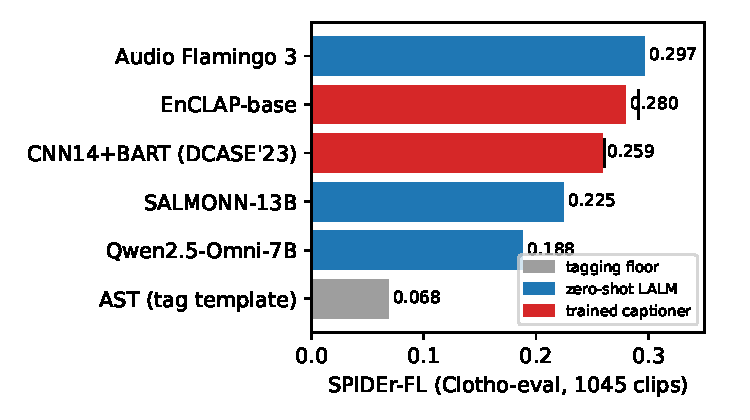
\includegraphics[width=\columnwidth]{fig1_spider_bar}
\caption{SPIDEr-FL on full Clotho-eval. Black ticks: published scores of the trained captioners.}
\label{fig:spider}
\end{figure}

\begin{table}[t]
\centering
\caption{SPIDEr-FL on the polyphonic vs.\ monophonic subsets ($\tau{=}0.25$; 336/709 clips).}
\label{tab:polymono}
\resizebox{\columnwidth}{!}{\IfFileExists{tables/table2_polymono.tex}{\begin{tabular}{lccc}
\toprule
Model & poly & mono & $\Delta$(poly$-$mono) \\
\midrule
AST (tag template) & 0.081 & 0.062 & +0.019 \\
Qwen2.5-Omni-7B & 0.250 & 0.157 & +0.094 \\
SALMONN-13B & 0.262 & 0.204 & +0.059 \\
CNN14+BART (DCASE'23) & 0.298 & 0.238 & +0.060 \\
EnCLAP-base & 0.329 & 0.256 & +0.073 \\
Audio Flamingo 3 & 0.356 & 0.268 & +0.088 \\
\bottomrule
\end{tabular}
% n_poly=336, n_mono=709
}{PENDING}}
\end{table}

\begin{table}[t]
\centering
\caption{CHAIR-audio caption-level hallucination rates (dual criterion).}
\label{tab:chair}
\resizebox{\columnwidth}{!}{\IfFileExists{tables/table3_chair.tex}{\begin{tabular}{lccc|c}
\toprule
Model & \multicolumn{3}{c|}{CHAIR-s at $\tau$} & coverage \\
 & 0.20 & \textbf{0.25} & 0.30 & ($\tau{=}0.25$) \\
\midrule
AST (tag template) & 0.952 & \textbf{0.956} & 0.968 & 1.00 \\
Qwen2.5-Omni-7B & 0.534 & \textbf{0.550} & 0.561 & 0.91 \\
SALMONN-13B & 0.322 & \textbf{0.332} & 0.337 & 0.80 \\
CNN14+BART (DCASE'23) & 0.343 & \textbf{0.350} & 0.358 & 0.75 \\
EnCLAP-base & 0.338 & \textbf{0.351} & 0.357 & 0.76 \\
Audio Flamingo 3 & 0.331 & \textbf{0.347} & 0.355 & 0.82 \\
\bottomrule
\end{tabular}
}{PENDING}}
\end{table}

\subsection{RQ1: Zero-Shot LALMs vs.\ Trained Captioners}
TODO %% ordering AST << Qwen < SALMONN < CNN14 < EnCLAP < AF3; H1 outcome.

\subsection{RQ2: Polyphonic vs.\ Monophonic}
TODO %% Table 2, H2 outcome with CIs.

\subsection{RQ3: Hallucination}
TODO %% Table 3; Qwen outlier; AST validity check; H3/H4 outcomes.

\section{Discussion and Limitations}\label{sec:discussion}
TODO %% overlap metrics reward reference-like phrasing; AST 10.24s window;
%% closed-vocab matcher misses synonyms (bias uniform across models, cancels
%% in paired comparisons); AudioSet ontology parents inflate polyphony.

\subsection{Deviations from the Preregistration}\label{sec:deviations}
TODO %% D1-D5 verbatim from the plan + never-frozen disclosure.

\section{Conclusion}\label{sec:conclusion}
TODO

\section*{AI Transparency Statement}
%% Required by course. Tools, versions, prompt categories, human verification.
TODO

\section*{Code and Data Availability}
Code, configs, run manifests, and all result files:
\url{https://github.com/Zuraiz270/audio-to-text-captioning-using-LALMs}.
Clotho v2.1 is publicly available; model checkpoints are cited in the repository.

\bibliographystyle{IEEEtran}
\bibliography{references}

\end{document}
